\documentclass[a4paper,12pt,abstracton]{scrartcl}
\usepackage[utf8]{inputenc}
\usepackage{float}
\usepackage{tikz}
\usepackage{amsmath}
\usepackage{amssymb}
\usepackage{pifont}% http://ctan.org/pkg/pifont
\usepackage[font=small,labelfont=bf]{caption}
\usepackage{graphicx}
\usepackage{dirtytalk}
\usepackage{multicol}
\usepackage{booktabs}
\usepackage{colortbl}
\usepackage{appendix}
\usepackage{nomencl}
\usepackage{lmodern}
\usepackage[nottoc]{tocbibind}
\usepackage{xcolor}
%\graphicspath{images/}
\usepackage[margin = 3cm]{geometry}
\usepackage{ragged2e} % good alignment
\usepackage{hyperref}
\usepackage{siunitx} % Provides the \SI{}{} and \si{} command for typesetting SI units
\hypersetup{colorlinks=true,
    linkcolor=blue,
    filecolor=magenta,      
    urlcolor=cyan, 
    citecolor=gray}

%\DeclareGraphicsExtensions{.png,.pdf} % low-res (work in progress)
%\DeclareGraphicsExtensions{.pdf,.png}  % high-res (final draft)
%\setlength\parindent{0pt} % Removes all indentation from paragraphs
%\bibliographystyle{unstr}
\setlength\parindent{0pt}
\setlength{\parskip}{0.3em}
\newcommand{\xmark}{\ding{55}}

\begin{document}
\section{Normal Zeeman Effect}

\subsection{Data Collection}

The data regarding the transverse and longitudinal configurations have been collected and reported in \hyperref[table:znt]{Table \ref*{table:znt}} and \hyperref[table:znl]{ \ref*{table:znl}} respectively. The values of $B$ have been derived from those of $I$ in \hyperref[sec:cal]{Calibration Curve}, while $\frac{\langle \delta \rangle}{\langle \Delta \rangle}$ has been calculated as described in \hyperref[sec:ExpIntro]{Experimental Introduction}.

\subsection{Data Analysis \& Visualization}

The datasets concerning the transverse and longitudinal configurations have been fit with the linear model $f(B)=\boldsymbol{p_0}B+\boldsymbol{p_1}$ and plotted in \hyperref[fig:znt]{Figure \ref*{fig:znt}} and \hyperref[fig:znl]{ \ref*{fig:znl}}, together with the respective fit parameters $\boldsymbol{p_0}$ and  $\boldsymbol{p_1}$ .


\begin{table}[H]
\centering
\caption{}
\label{table:znt}
\resizebox{8cm}{!}{
  \begin{tabular}{cccccc}
  \toprule
 $I\;[A]$ & $B\;[T]$ & $\frac{\langle \delta \rangle}{\langle \Delta \rangle}$ \\
  \midrule
  \rowcolor{gray!6}  2.61 $\pm$ 0.02 & 0.183 $\pm$ 0.019 & 0.061 $\pm$ 0.004\\
  4.92 $\pm$ 0.02 & 0.338 $\pm$ 0.035 & 0.125 $\pm$ 0.007\\
  \rowcolor{gray!6}  5.84 $\pm$ 0.02 & 0.400 $\pm$ 0.041 & 0.158 $\pm$ 0.003\\
  6.83 $\pm$ 0.02 & 0.466 $\pm$ 0.048 & 0.188 $\pm$ 0.006\\
  \rowcolor{gray!6}  7.225 $\pm$ 0.025 & 0.500 $\pm$ 0.052 & 0.198 $\pm$ 0.006\\
  7.92 $\pm$ 0.02 & 0.543 $\pm$ 0.056 & 0.221 $\pm$ 0.004\\
  \rowcolor{gray!6}  8.91 $\pm$ 0.02 & 0.596 $\pm$ 0.062 & 0.233 $\pm$ 0.006\\
  9.92 $\pm$ 0.02 & 0.641 $\pm$ 0.066 & 0.263 $\pm$ 0.009\\
  \bottomrule
   \addlinespace
  \end{tabular}}
\end{table}

\begin{figure}[H]
    \centering
    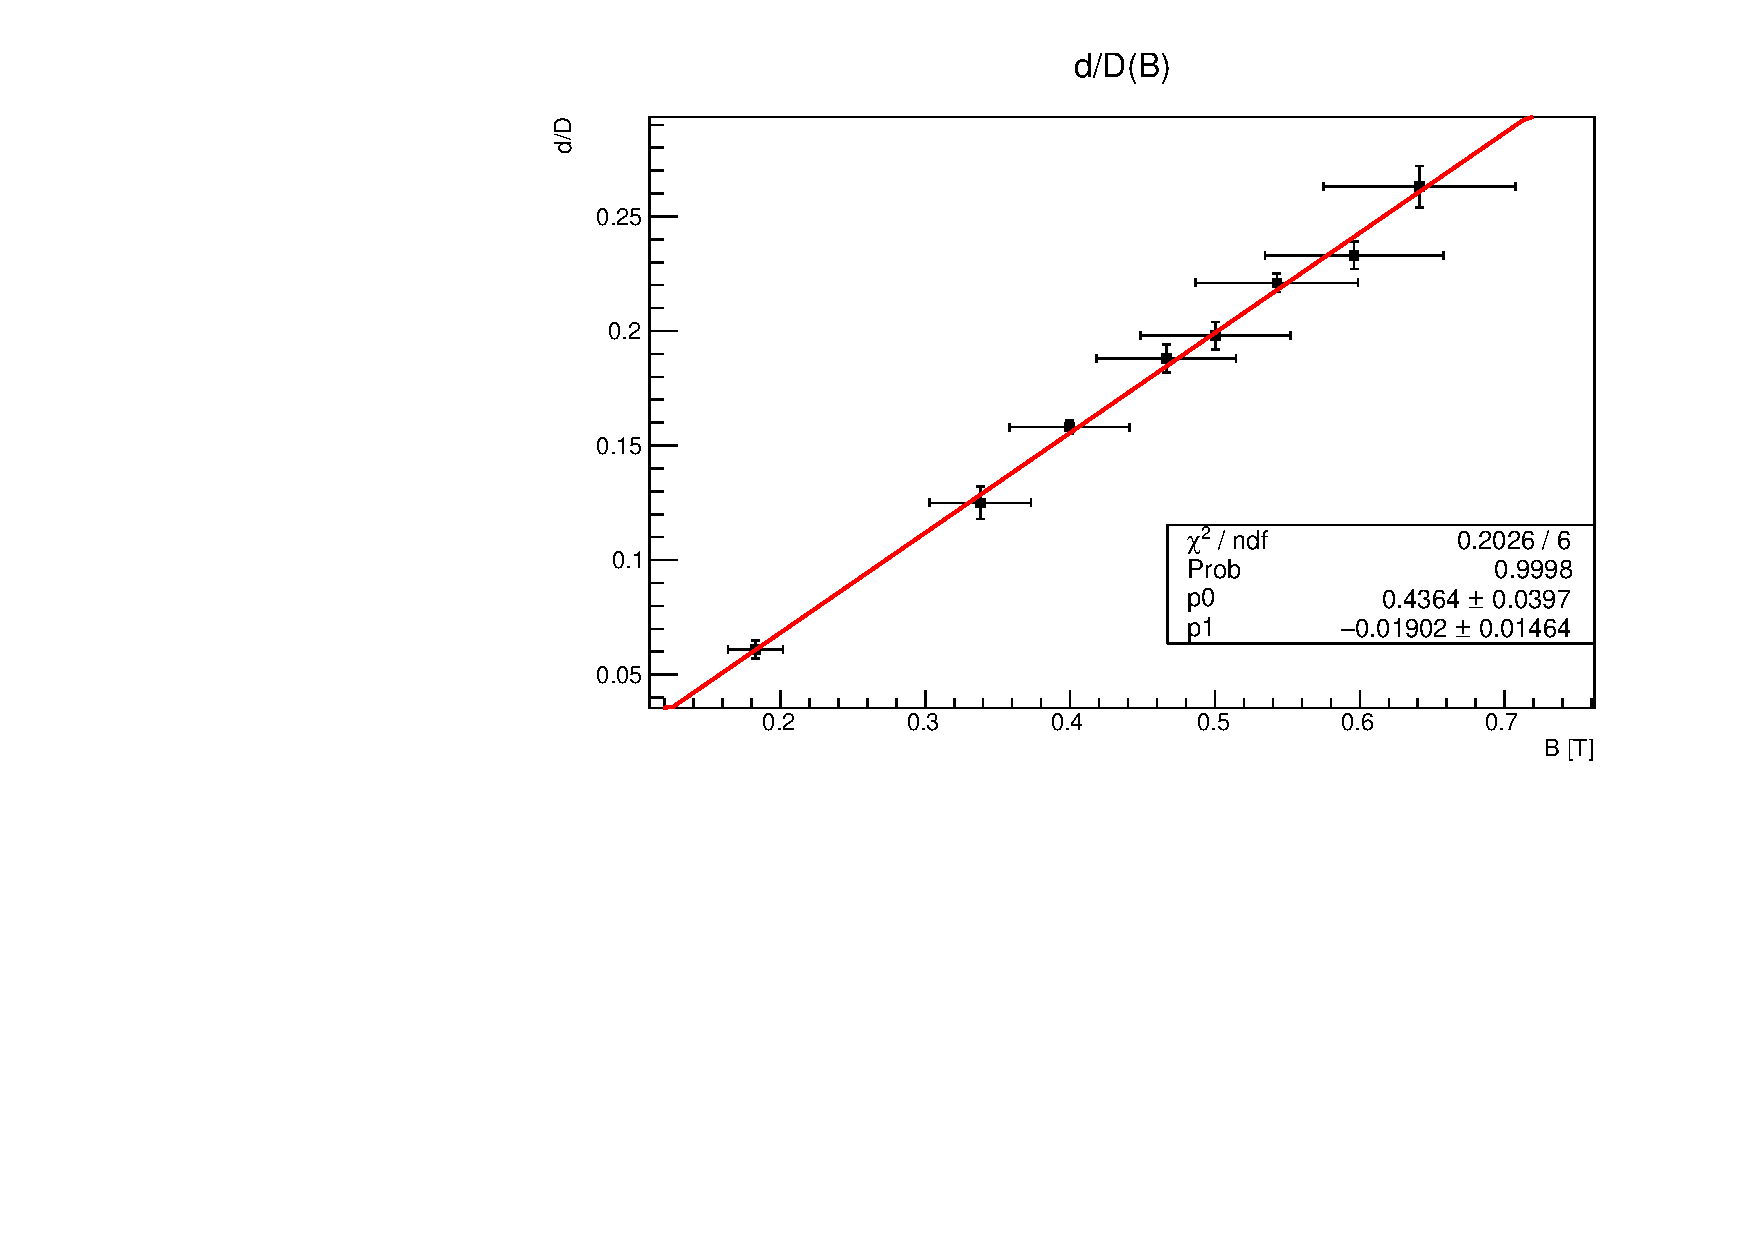
\includegraphics[scale=0.66]{plots/znt.pdf}
    \caption{Transverse}
    \label{fig:znt}
\end{figure}


\begin{table}[H]
\centering
\caption{}
\label{table:znl}
\resizebox{12cm}{!}{
  \begin{tabular}{cccccc}
  \toprule
 $I\;[A]$ & $B\;[T]$ & $\frac{\langle \delta \rangle}{\langle \Delta \rangle}$ \\
  \midrule
  \rowcolor{gray!6}  2.69 $\pm$ 0.02 & 0.188 $\pm$ 0.019 & 0.070 $\pm$ 0.002\\
  4.84 $\pm$ 0.02 & 0.333 $\pm$ 0.034 & 0.140 $\pm$ 0.003\\
  \rowcolor{gray!6}  5.91 $\pm$ 0.02 & 0.404 $\pm$ 0.082 & 0.165 $\pm$ 0.002\\
  6.93 $\pm$ 0.03 & 0.473 $\pm$ 0.049 & 0.192 $\pm$ 0.002\\
  \rowcolor{gray!6}  7.23 $\pm$ 0.02 & 0.500 $\pm$ 0.052 & 0.202 $\pm$ 0.010\\
  7.86 $\pm$ 0.02 & 0.539 $\pm$ 0.056 & 0.218 $\pm$ 0.002\\
  \rowcolor{gray!6}  8.83 $\pm$ 0.02 & 0.592 $\pm$ 0.061 & 0.237 $\pm$ 0.006\\
  9.80 $\pm$ 0.02 & 0.636 $\pm$ 0.066 & 0.263 $\pm$ 0.009\\
  \bottomrule
  \addlinespace
    \addlinespace
  \addlinespace
  \addlinespace
  \addlinespace
  \addlinespace
  \addlinespace
   \addlinespace
  \end{tabular}}
\end{table}

\begin{figure}[H]
    \centering
    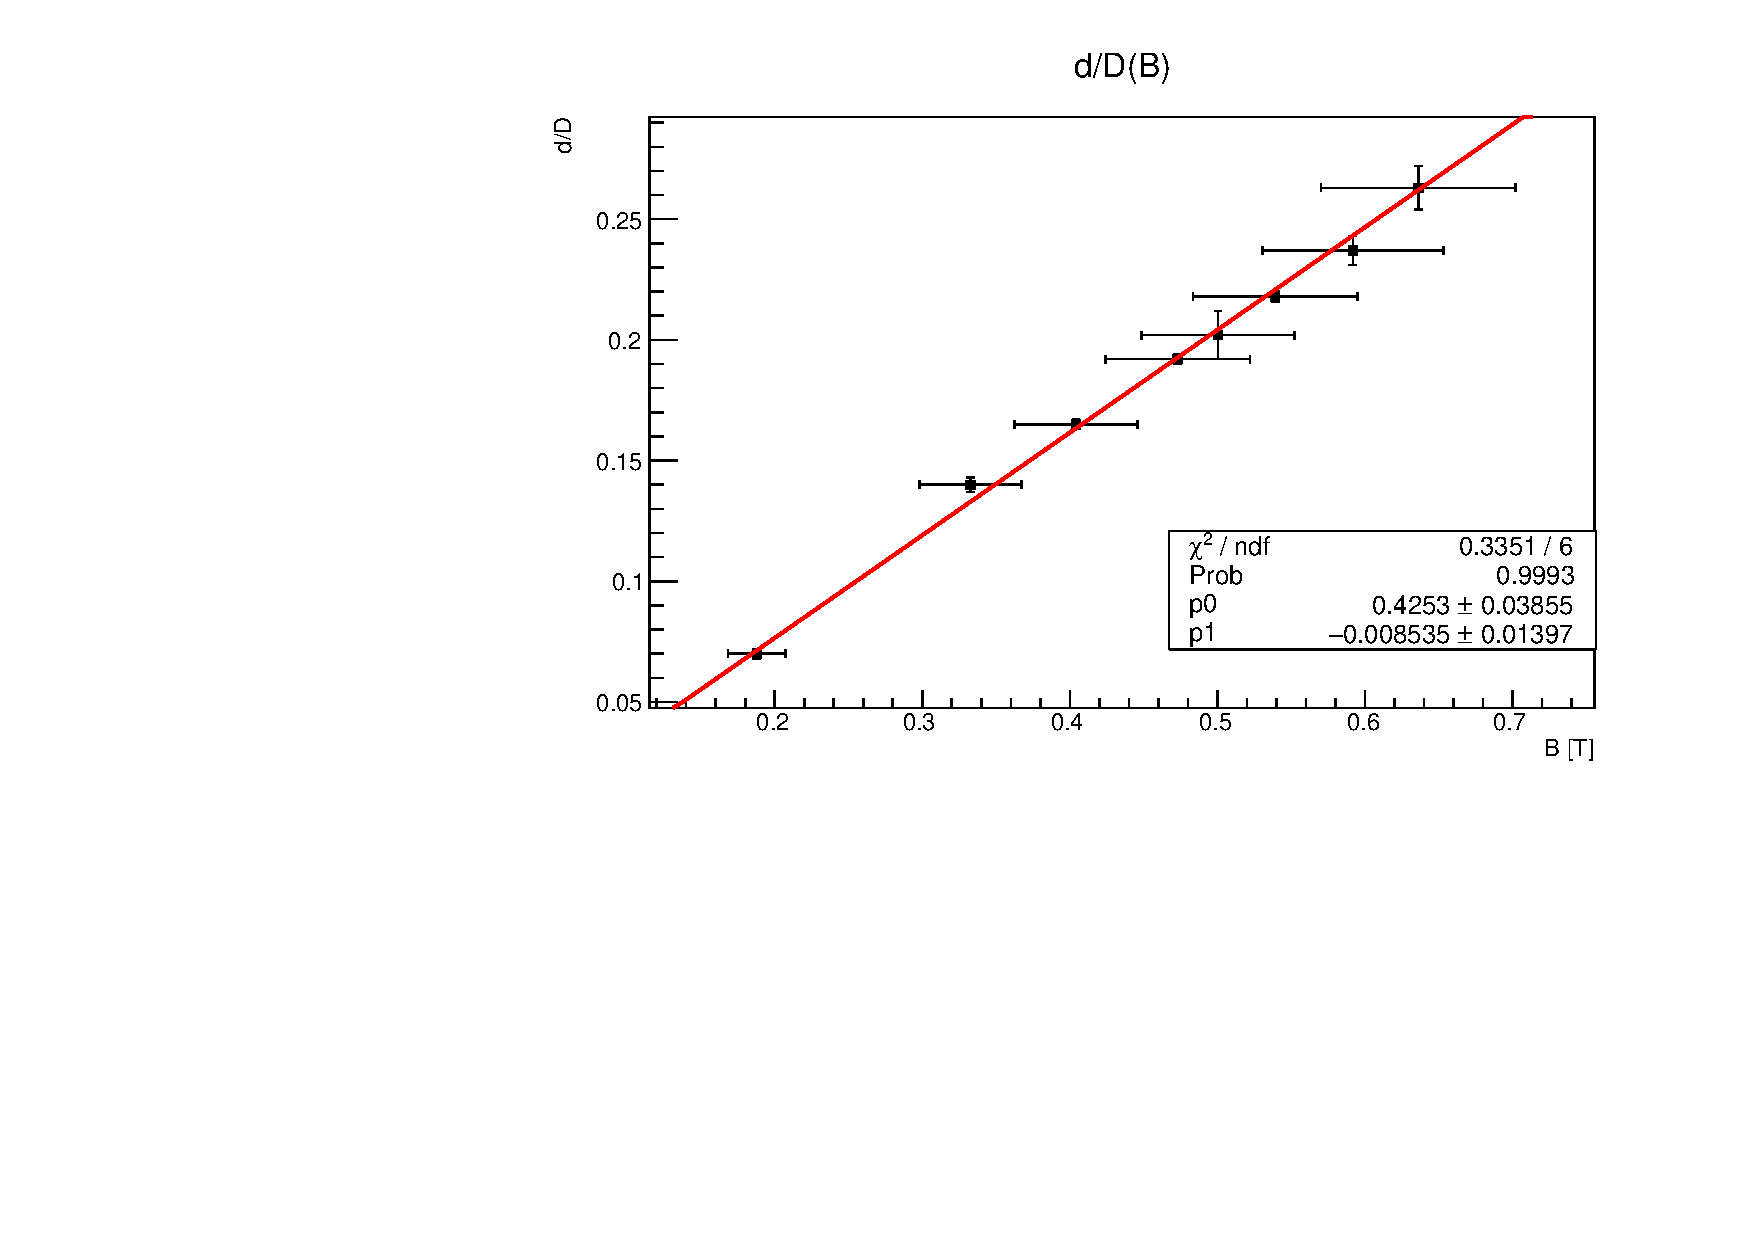
\includegraphics[scale=0.85]{plots/znl.pdf}
    \caption{Longitudinal}
    \label{fig:znl}
\end{figure}
        
\clearpage

\subsection{Bohr Magneton}
Now it is possible to calculate the Bohr magneton for both configurations $$\mu_N^T= (\boldsymbol{p_0^T}\pm \boldsymbol{\delta p_0^T})\frac{hc}{2g_n\mu_n w} \quad\text{and}\quad \mu_N^L= (\boldsymbol{p_0^L}\pm \boldsymbol{\delta p_0^L})\frac{hc}{2g_n\mu_n w}$$ 
 since we know 
\begin{itemize}
\item $h=6.626070040\times10^{-34} \text{ Js}  \;\,\quad\qquad\qquad\text{ Plack constant}$  
\item $c=299792458 \text{ ms}^{-1}  \quad\qquad\qquad\qquad\qquad\text{speed of light in the vacuum}$
\item $g_n=1   \;\;\qquad\qquad\qquad\qquad\qquad\qquad\qquad\text{ gyromagnetic factor}$
\item $\mu_n= 1.4560    \;\qquad\qquad\qquad\qquad\qquad\qquad\text{ refractive index}$
\item  $w= 0.003 \text{ m} \;\qquad\qquad\qquad\qquad\qquad\qquad\text{thickness}$
\item $\boldsymbol{p_0^{T}}=0.436 \pm 0.040 \;\text{T}^{-1} \;\quad\qquad\qquad\qquad\text{ transverse slope}$
\item $\boldsymbol{p_0^{L}}=0.425 \pm 0.039 \;\text{T}^{-1} \;\quad\qquad\qquad\qquad\text{ longitudinal slope .}$\newline
\end{itemize}
The compatibility between $\mu_N^T$ and $\mu_N^L$ has been tested as displayed in \hyperref[table:Zn]{Table \ref*{table:Zn}}. 
\begin{table}[H]
\caption{}
\centering
\resizebox{10cm}{!}{
\begin{tabular}{cccc}
\toprule
$\mu_N^T\;[\text{JT}^{-1}]$ & $\mu_N^L\;[\text{JT}^{-1}]$ & $Z$ & Compatibility  \\
\midrule
\rowcolor{gray!6} $9.91 \pm  0.91\times 10^{-24}$ & $9.66 \pm  0.89\times 10^{-24}$ & 0.20 & \checkmark \\
\bottomrule
\end{tabular}}
\label{table:Zn}
\end{table}

Since the result has been positive, we have calculated the weighted average $ \langle \mu_N\rangle$ and tested against the theoretical value $\boldsymbol{\mu_B}$ as shown in \hyperref[table:ZnT]{Table \ref*{table:ZnT}} .

\begin{table}[H]
\caption{}
\centering
\resizebox{10cm}{!}{
\begin{tabular}{cccc}
\toprule
$\langle \mu_N \rangle \;[\text{JT}^{-1}]$ & $\boldsymbol{\mu_B} \;[\text{JT}^{-1}]$ & $Z$ & Compatibility  \\
\midrule
\rowcolor{gray!6} $9.79 \pm 0.63 \times 10^{-24}$ & $9.27 \times 10^{-24}$ & 0.41 & \checkmark \\
\bottomrule
\end{tabular}}
\label{table:ZnT}
\end{table}


\clearpage
\end{document}
